
\documentclass{beamer}
\usetheme{metropolis}           % Use metropolis theme
\title{Heavy lake-effect snowfall events for the Laurentian Great Lakes region for current and future climates}
\date{July 2019}
\author{O. Huziy\textsuperscript{1,2,3} and L. Sushama\textsuperscript{2}, L. Leon\textsuperscript{3}, R. Yerubandi\textsuperscript{3}}
\institute{
  \textsuperscript{1}Environement and Climate Change Canada,\\
  \textsuperscript{2}McGill University,\\
  \textsuperscript{3}Université du Québec à Montréal
}

\graphicspath{{figures/}}
\usepackage[export]{adjustbox}
\usepackage{array}
\newcommand{\logovspace}{0.5cm}
\usepackage{natbib}[plain]
\renewcommand*{\bibfont}{\footnotesize}

\renewcommand\bibname{}
\renewcommand\refname{}


\begin{document}
  \maketitle

  \begin{frame}{Outline}
    \begin{itemize}
      \item Motivation and previous work
      \item Methods
      \begin{itemize}
        \item Models and simulation configurations
        \item Heavy Lake Effect Snowfall (HLES) search algorithm
      \end{itemize}

      \item Results
      \begin{itemize}
        \item HLES in current climate, validation
        \item Projected changes to HLES
      \end{itemize}
    \end{itemize}
  \end{frame}

  \section{Motivation and previous work}
  \begin{frame}{Objectives}
    \begin{itemize}
      \item Apply a more advanced tool to study projected changes to HLES in the Great Lakes region: coupled GEM(atm)-NEMO(lake) system.
      \item Look into how HLES is going to change during different sub-seasons of the cold season: ND, JF, MA.
      \item Study links between HLES and other near-surface and surface fields: temperature, precipitation, ice concentration in current and future climate.
    \end{itemize}
  \end{frame}

  \section{Models and simulation configurations}
  \begin{frame}{Models and simulation configurations}
    \begin{columns}[T]
      \column{0.5\textwidth}
          \includegraphics[width=\textwidth]{{sim_domain_and_focus_region}.png}


      \column{0.5\textwidth}
        Specify GEM and NEMO options relevant for HLES.
    \end{columns}



  \end{frame}

  \section{HLES in current climate}
  \begin{frame}{Validation}

      \begin{figure}
        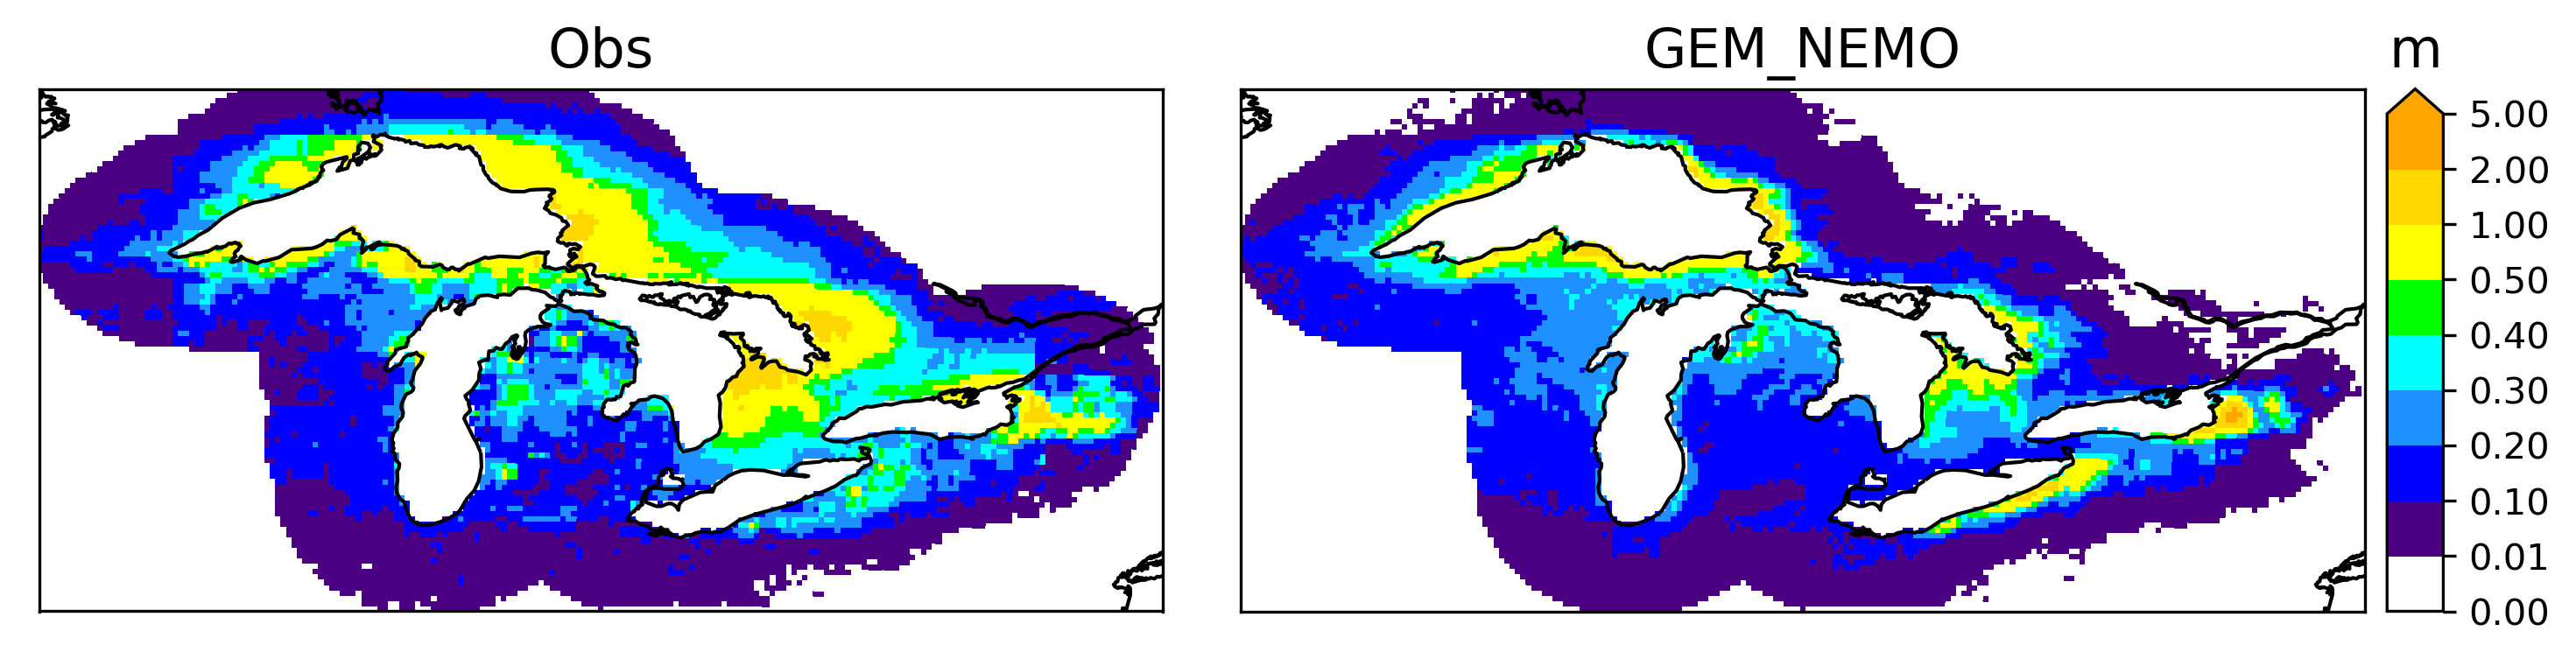
\includegraphics[width=0.8\textwidth]{hles_clim_snow_fall_1980-2009.png}
        \caption{\footnotesize Mean cold season HLES (m)}
      \end{figure}

      \begin{columns}
        \column{0.5\textwidth}
          \begin{figure}
            \includegraphics[height=0.4\textheight]{{hles_histo_all_m9_10_11_12_1_2_3_4_5}.png}
            \caption{\footnotesize Monthly distribution of area-average HLES}
          \end{figure}


        \column{0.5\textwidth}
          \begin{itemize}
            \item Extent of HLES is mostly underestimated in GEM\_NEMO
            \item Overestimation downwind of lake Erie
            \item
          \end{itemize}
      \end{columns}


  \end{frame}


  \section{Projected changes to HLES}
  \begin{frame}{Projected changes to the fields impacting HLES}
    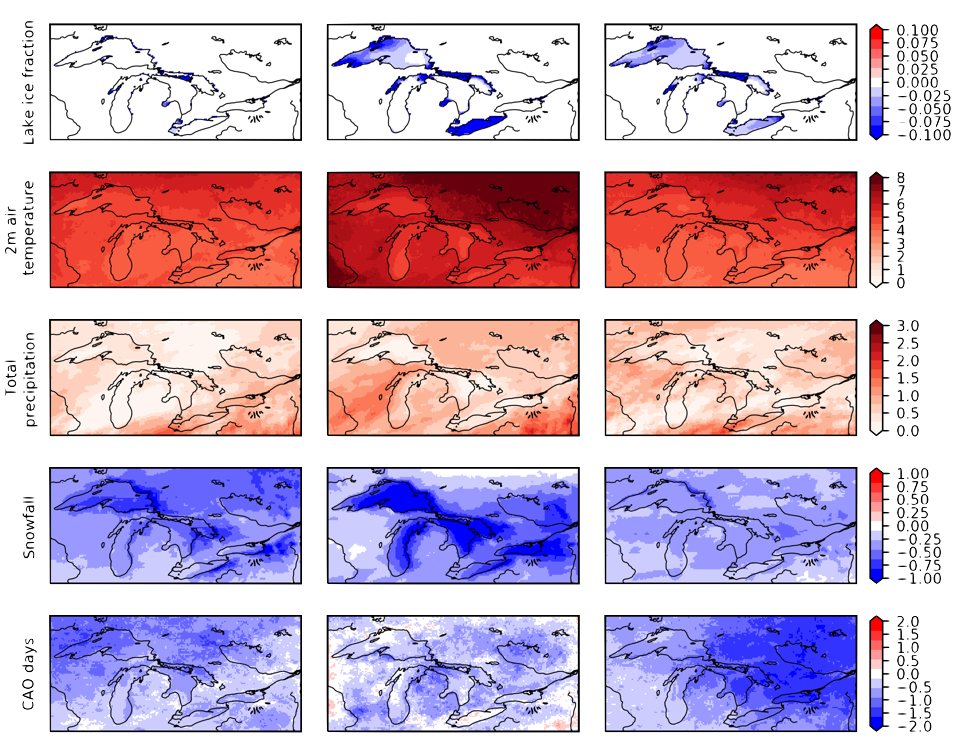
\includegraphics[height=0.9\textheight]{projected_changes_to_surf_and_nearsurf_fields.png}
  \end{frame}

  \begin{frame}{Projected changes to HLES: magnitudes and frequencies}
    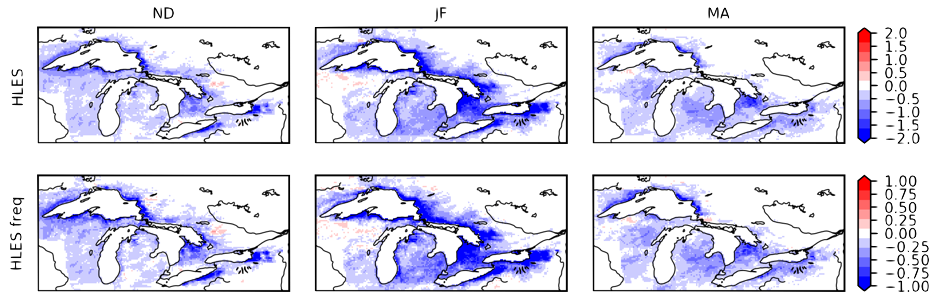
\includegraphics[width=\textwidth]{projected_changes_to_hles.png}
    \begin{itemize}
      \item TODO: summary
    \end{itemize}
  \end{frame}



%% No section here
  \begin{frame}{Conclusions}
    todo
  \end{frame}



  \begin{frame}{References}
    \nocite{*}
    \bibliographystyle{apa}
    \bibliography{references}


    todo
    \begin{itemize}
      \item Vavrus et al 2014
      \item GEM/CRCM reference
      \item NEMO reference
    \end{itemize}
  \end{frame}


  \begin{frame}{Acknowledgements}
      \centering
      \Large{Thanks to} \\[\logovspace]
      \small
      \begin{tabular} {m{14em} l}
        \includegraphics[height=1cm]{{nserc_logo}.png} & funding \\[\logovspace]
        \includegraphics[width=10em]{{computecanada_logo}.png}  & computing and storage resources \\[\logovspace]
        \includegraphics[width=5.5em]{{mcgill_logo}.png} \includegraphics[width=4.5em]{{logo_uqam}.png} & base universities   \\[\logovspace]
        \includegraphics[width=14em]{{eccc_logo}.png} & models, libraries and tools \\[\logovspace]
        M. Valin, K. Winger, B. Dugas, F. Dupont and other colleagues & for their help with the project
      \end{tabular}
  \end{frame}


  \begin{frame}[standout]
    Questions?
  \end{frame}

\appendix





\end{document}
